% Appendix Template

\chapter{Messaufbau} % Main appendix title

\label{AppendixD} % Change X to a consecutive letter; for referencing this appendix elsewhere, use \ref{AppendixX}

Die Kamera wurde jeweils an der Seite des Fahrzeugs mit Blick in Fahrtrichtung und dem Vorderrad im Bildbereich befestigt, wie die folgenden Fotos zeigen.

\begin{figure}[h]
    \centering
    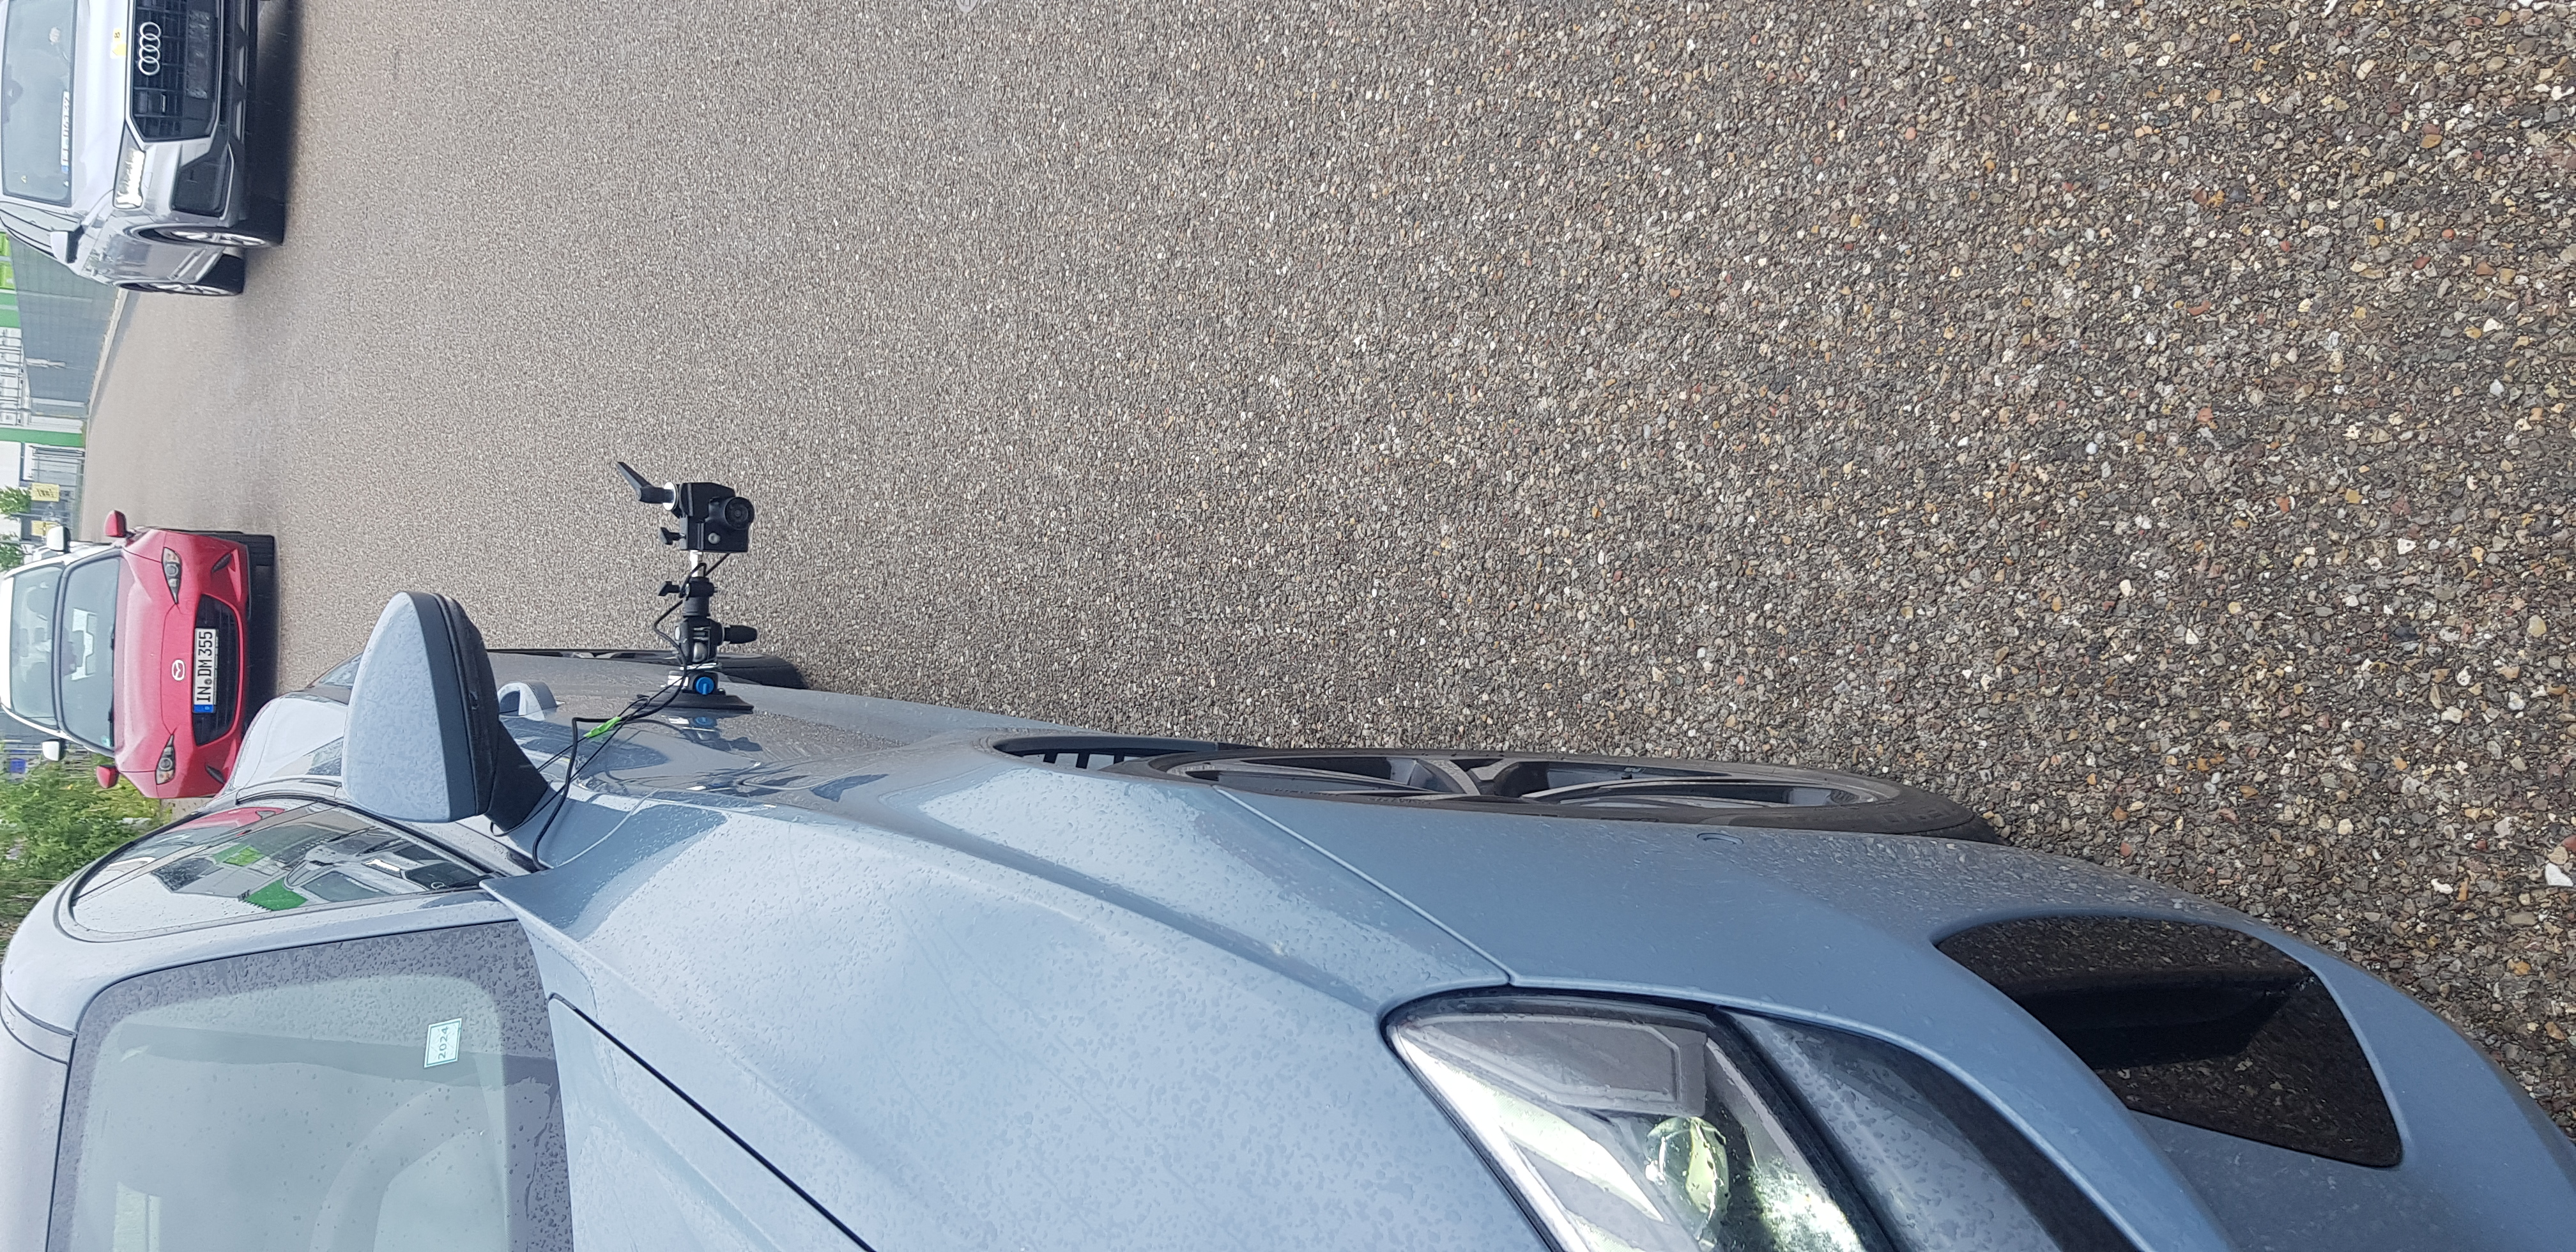
\includegraphics[width=\linewidth, angle=270]{Figures/Messaufbau/20250602_103722.jpg}
    \caption{Messaufbau Fahrerseite von vorn}
    \label{fig:Messaufbau_links_vorn}
\end{figure}
\begin{figure}[h]
    \centering
    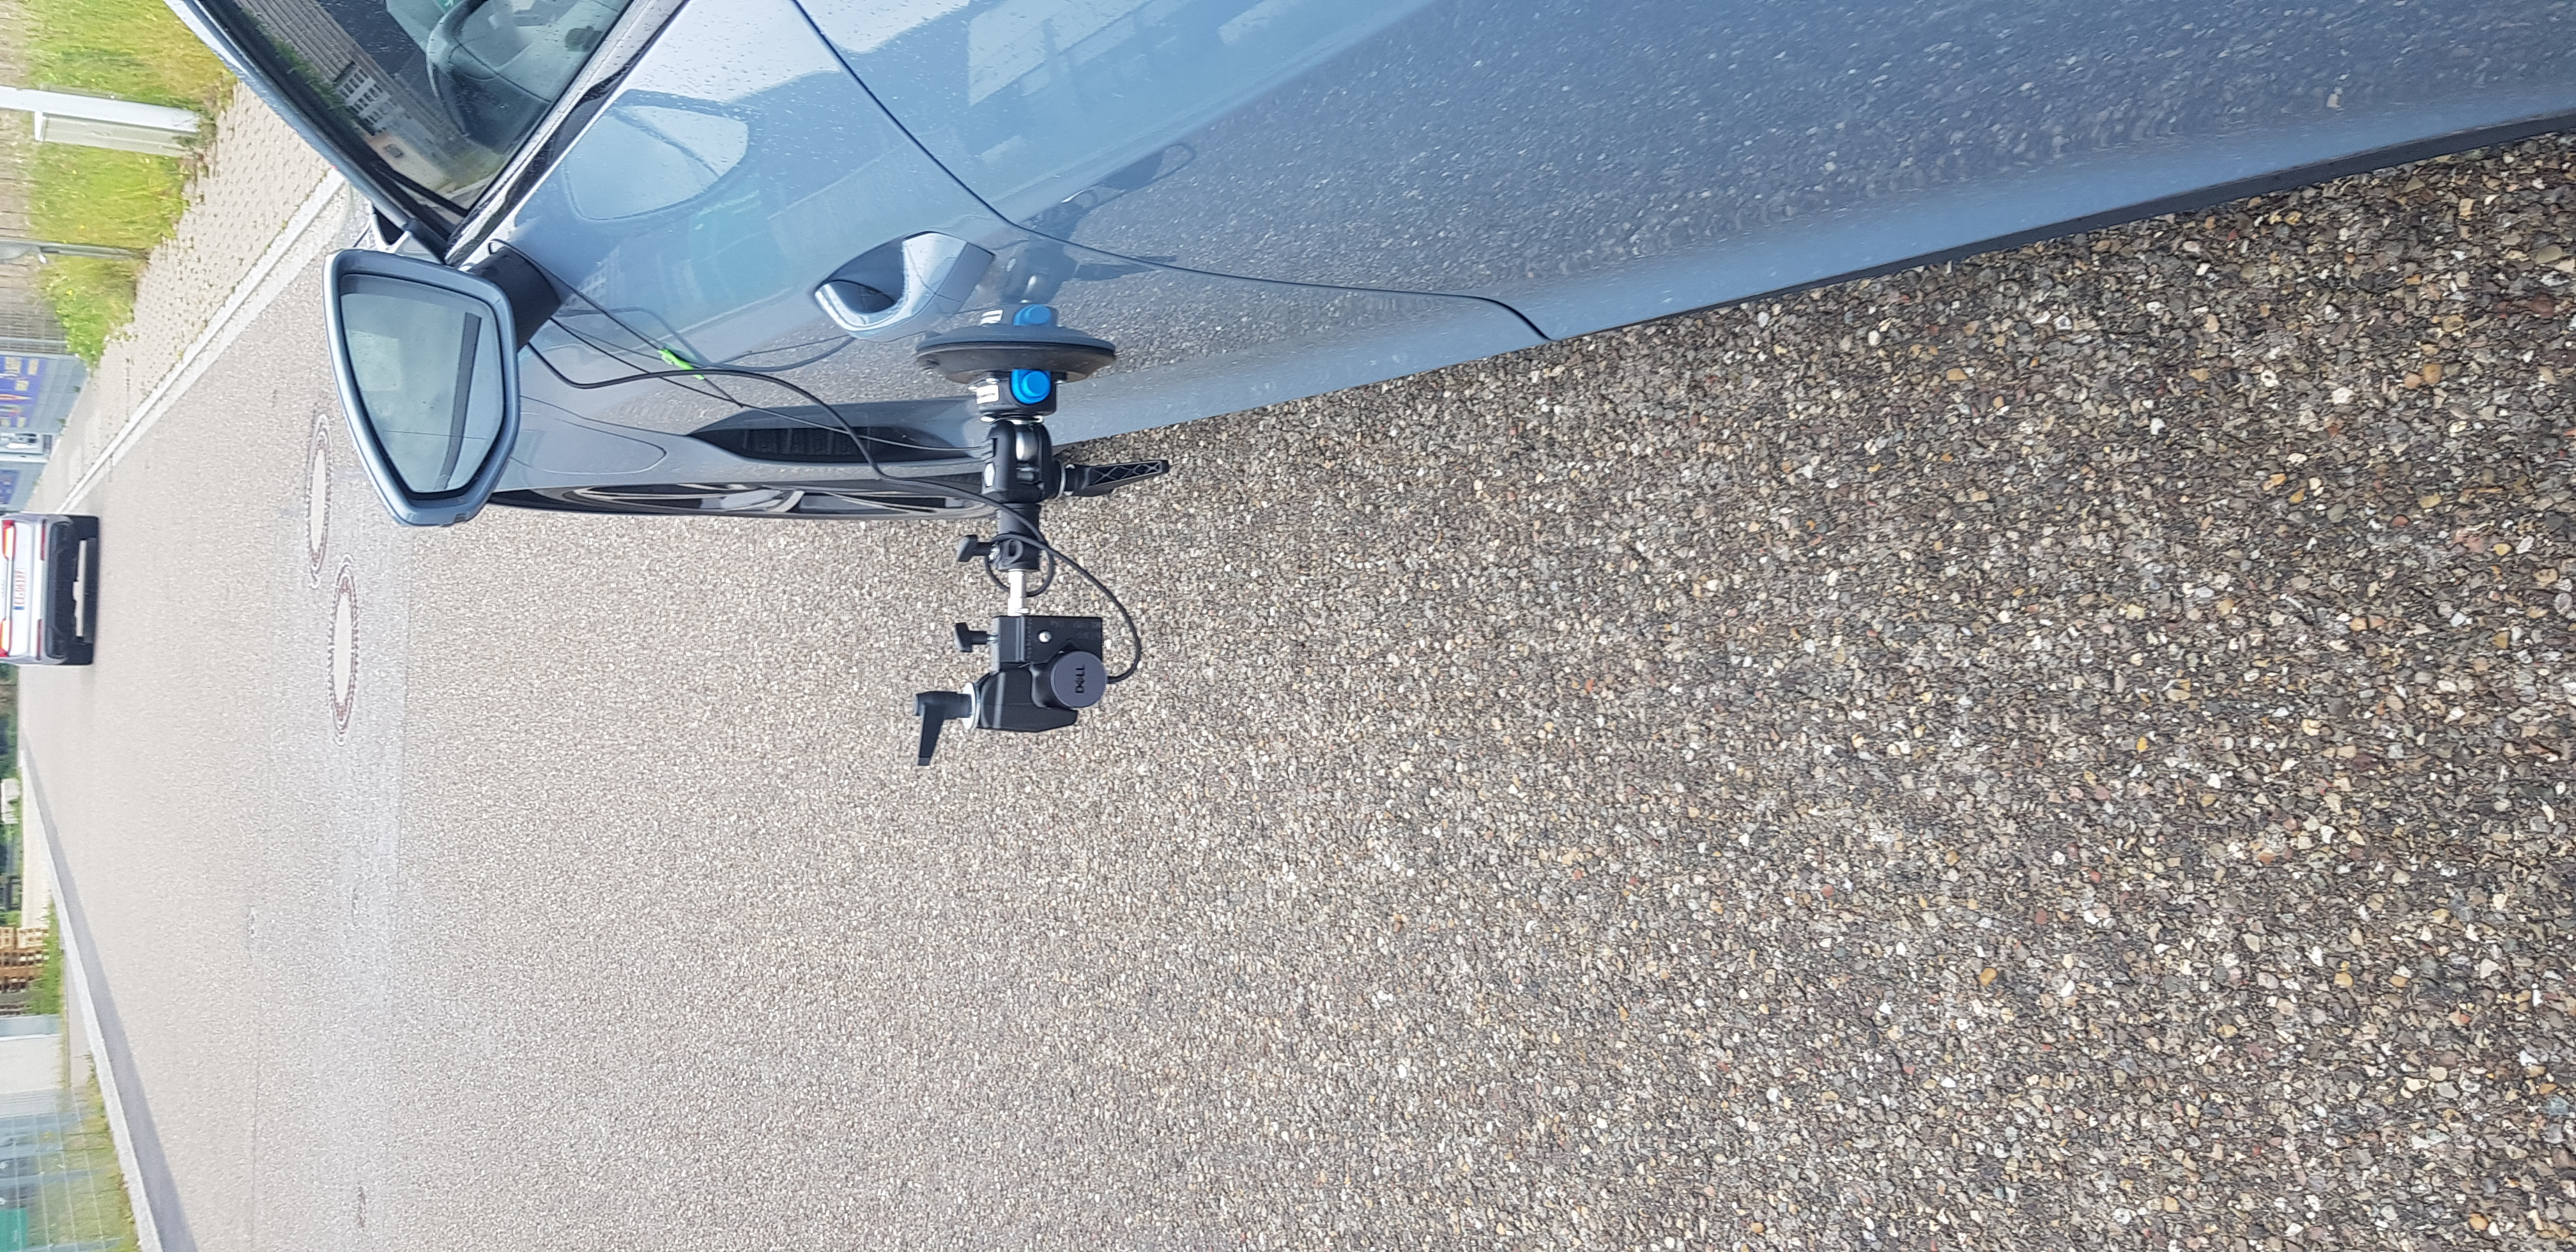
\includegraphics[width=\linewidth, angle=270]{Figures/Messaufbau/20250602_103736.jpg}
    \caption{Messaufbau Fahrerseite von hinten}
    \label{fig:Messaufbau_links_hinten}
\end{figure}
\begin{figure}[h]
    \centering
    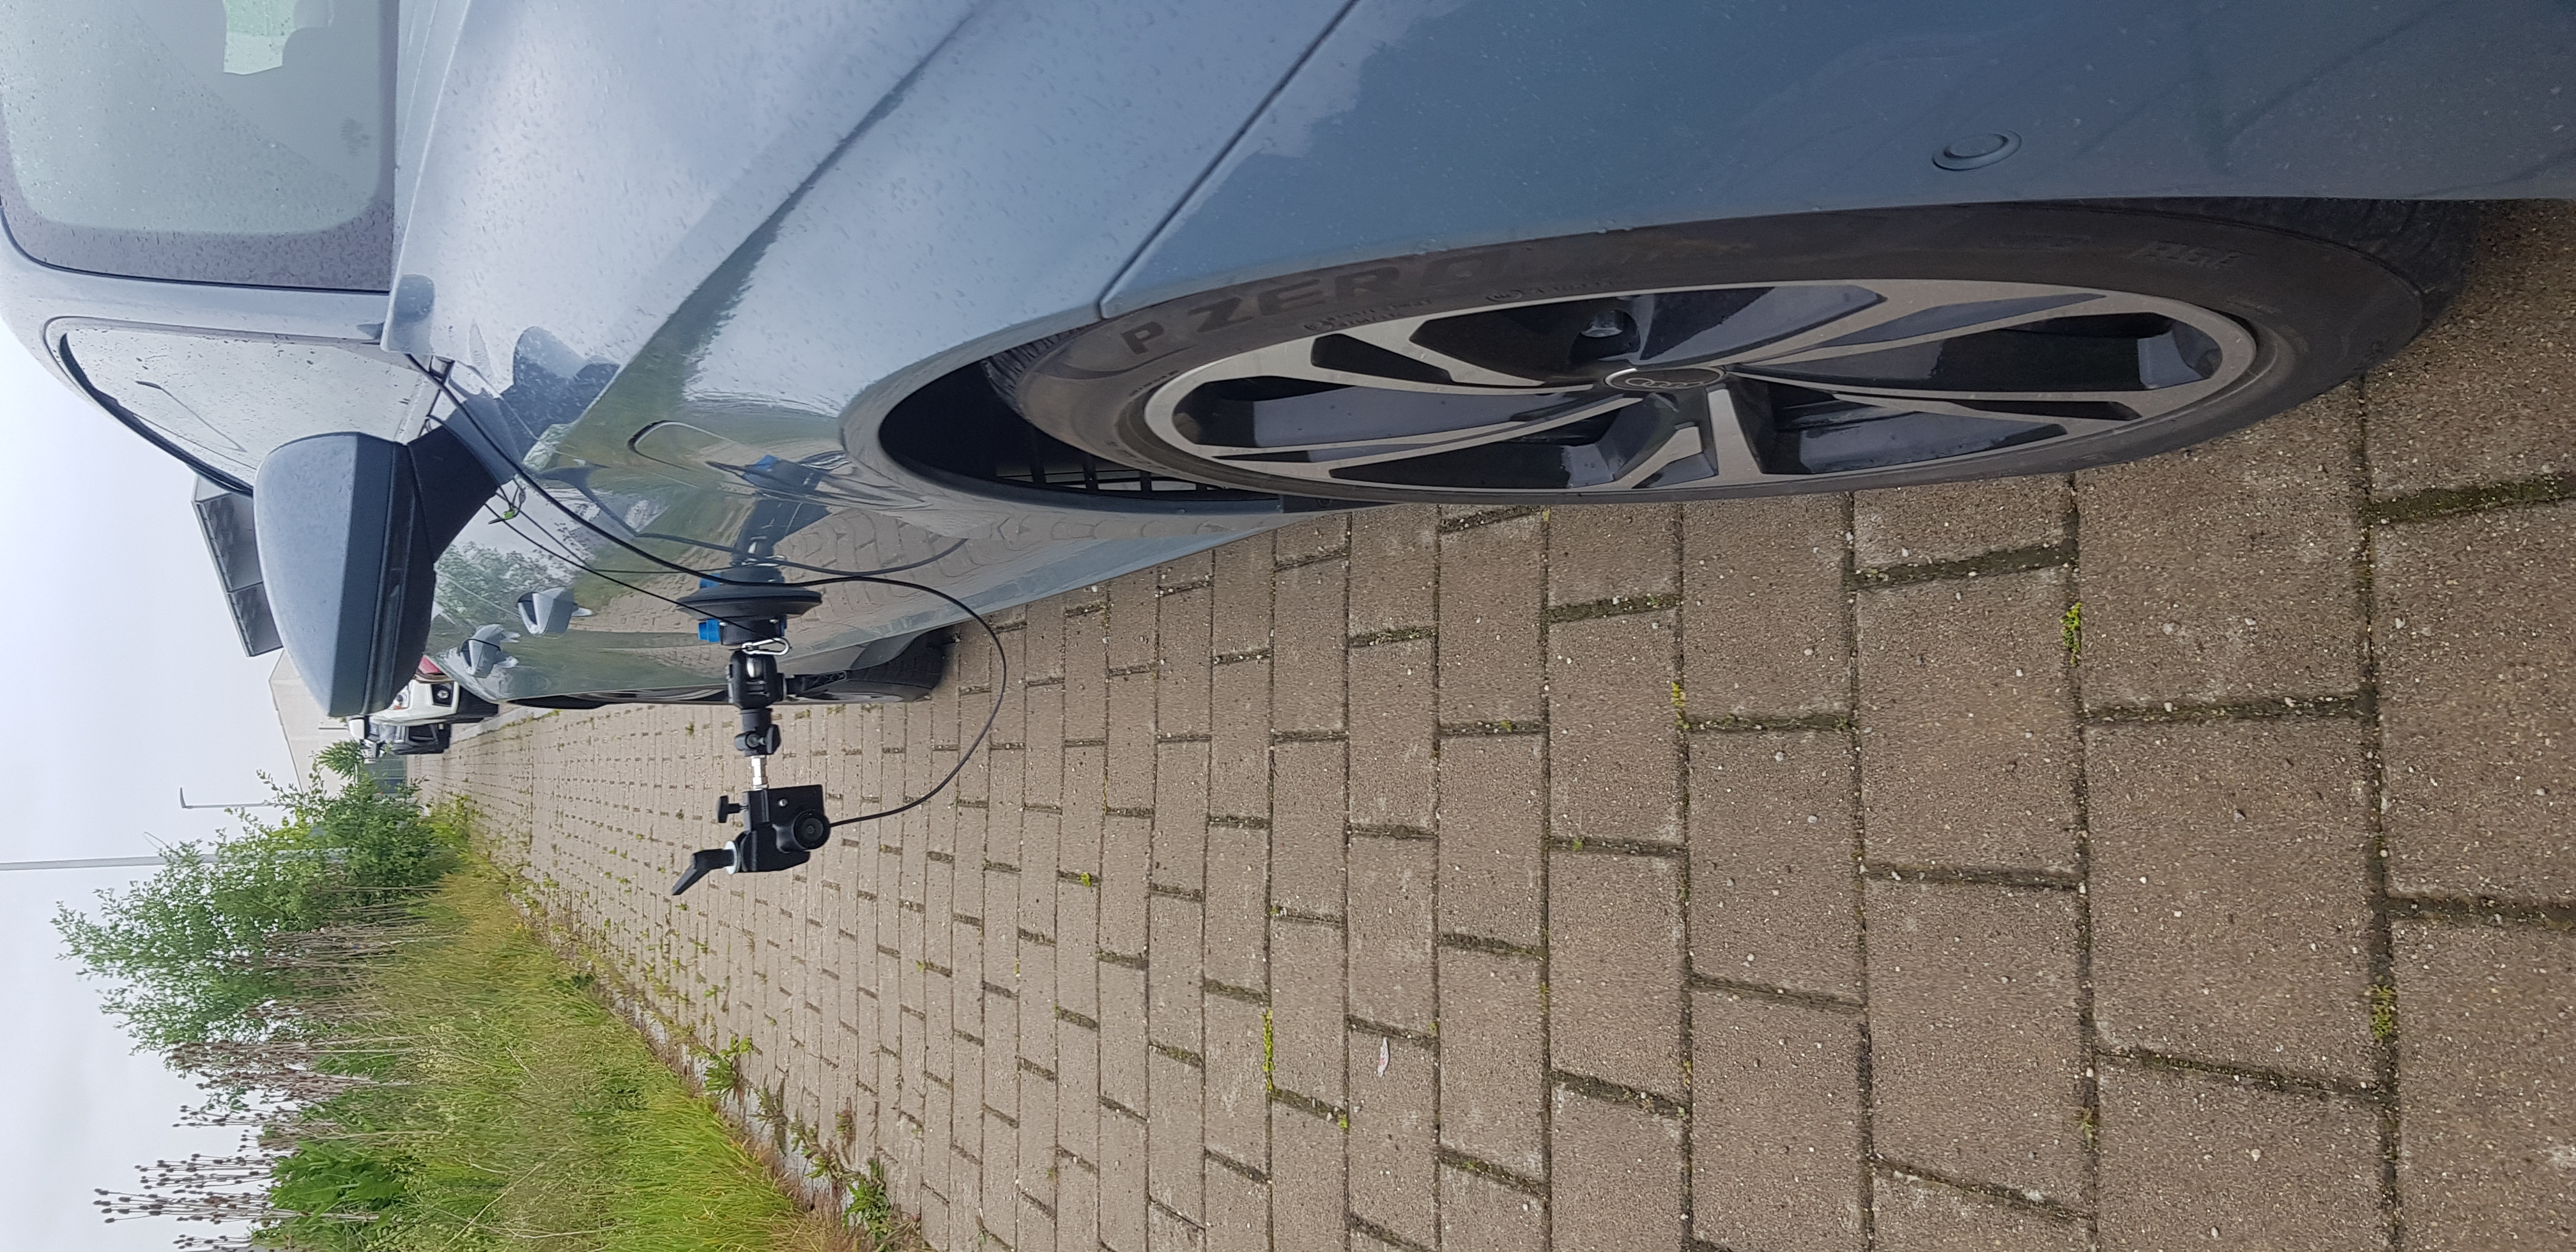
\includegraphics[width=\linewidth, angle=270]{Figures/Messaufbau/20250602_103752.jpg}
    \caption{Messaufbau Beifahrer von vorn}
    \label{fig:Messaufbau_rechts_vorn}
\end{figure}
\begin{figure}[h]
    \centering
    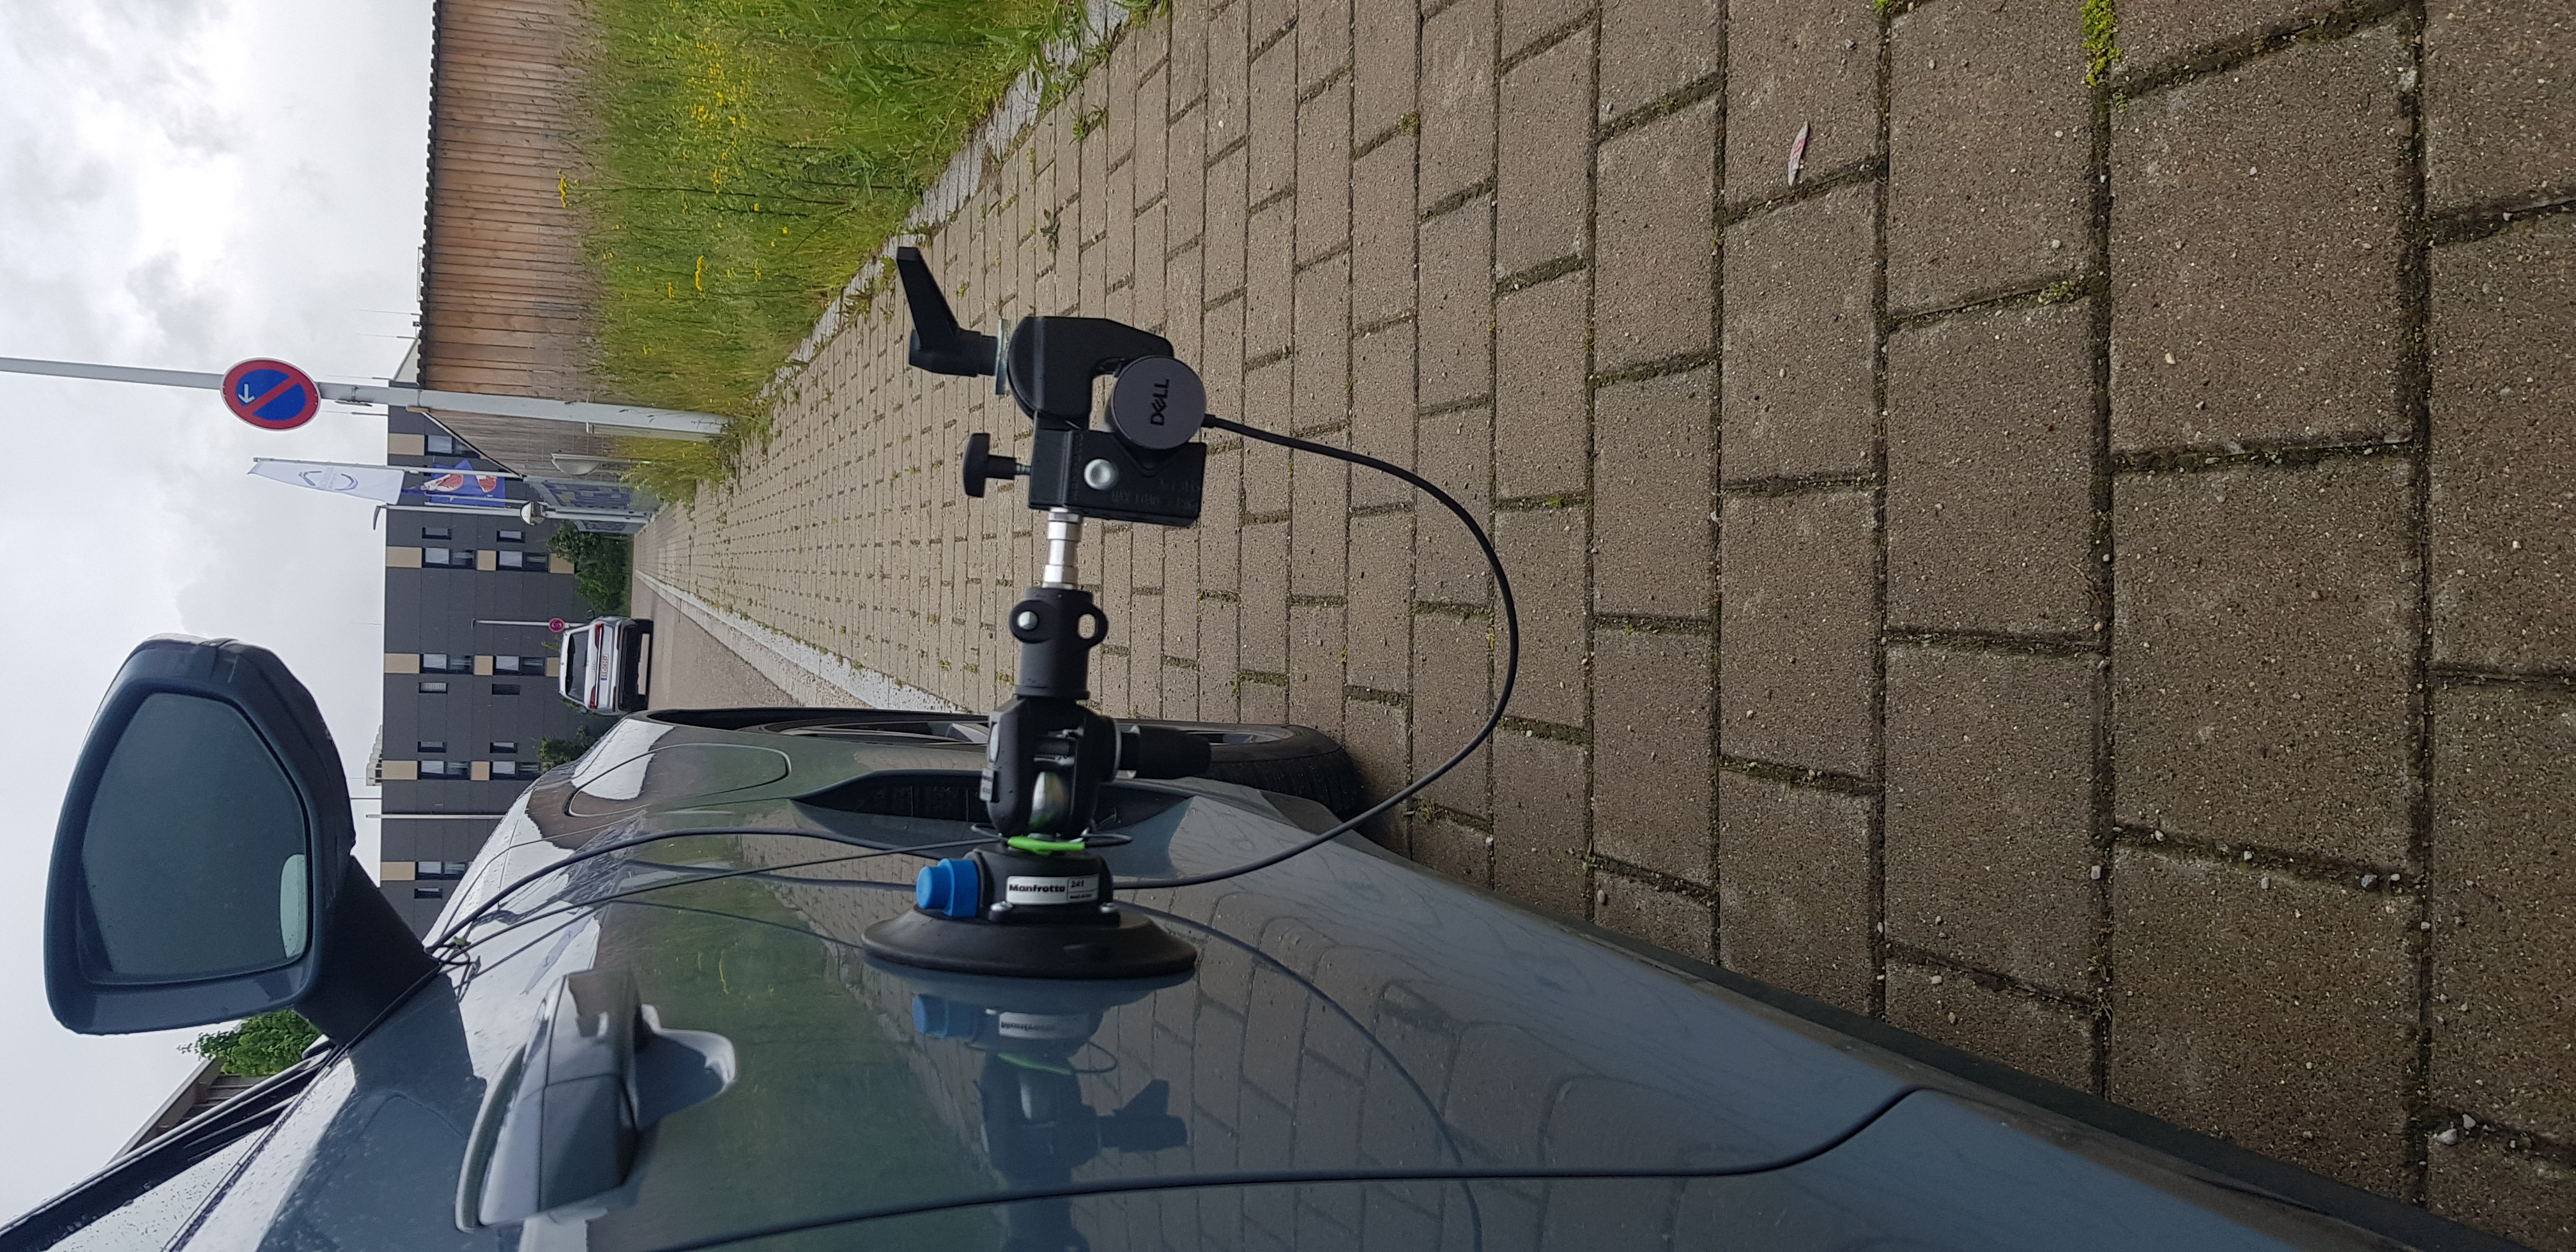
\includegraphics[width=\linewidth, angle=270]{Figures/Messaufbau/20250602_103801.jpg}
    \caption{Messaufbau Beifahrer von hinten}
    \label{fig:Messaufbau_rechts_hinten}
\end{figure}